    % IEEE standard conference template; to be used with:
%   spconf.sty  - LaTeX style file, and
%   IEEEbib.bst - IEEE bibliography style file.
% --------------------------------------------------------------------------

\documentclass[letterpaper]{article}

\usepackage{spconf,amsmath,amssymb,graphicx,amsthm,newlfont,program,caption,subcaption}
\usepackage[nodayofweek,level]{datetime}
\usepackage{textcomp}
%\usepackage[hyphens]{url}
\usepackage[hyphens]{url}
\usepackage{hyperref}

% Example definitions.
% --------------------
% nice symbols for real and complex numbers
%\newcommand{\R}[0]{\mathbb{R}}
%\newcommand{\C}[0]{\mathbb{C}}


% bold paragraph titles
\newcommand{\mypar}[1]{{\bf #1.}}

\theoremstyle{definition}
\newtheorem{observation}{Observation}

\newtheorem{algorithm}{Algorithm}

%\PassOptionsToPackage{hyphens}{url}\usepackage{hyperref}


% Title.
% ------
% TODO: think about it
\title{Parallel algorithms for finding the convex hull of a sorted point set}
%
% Single address.
% ---------------
\name{ Marek \v Cerv\'ak, Lorenzo Martini, Aleksander Matusiak} 
\address{Department of Computer Science\\ ETH Z\"urich\\Z\"urich, Switzerland}

% For example:
% ------------
%\address{School\\
%		 Department\\
%		 Address}
%
% Two addresses (uncomment and modify for two-address case).
% ----------------------------------------------------------
%\twoauthors
%  {A. Marek \v Cerv\'ak, B. Lorenzo Martini}
%		 {School A-B\\
%		 Department A-B\\
%		 Address A-B}
%  {C. Aleksander Matusiak}
%		 {School C-D\\
%		 Department C-D\\
%		 Address C-D}


\begin{document}
%\ninept
%
\maketitle
%

\begin{abstract}
The problem of computing the 2D convex hull of a set of points finds practical applications in many different fields, like pattern recognition, image processing and statistics.
The main contribution of this paper is to review some available parallel algorithms for computing the convex hull of a sorted set of points in the plane in the PRAM shared memory model.
We provide their implementation and evaluate their performance using high number of threads on a system mounting Intel Xeon Phi coprocessors.
Experimental results show that speedup for our implementations increases up to 128 processors.
For lower number of threads (up to 16) we also achieved superlinear speedup.

\textbf{Keywords:} Parallel Convex Hull, Shared memory, Xeon Phi.

\end{abstract}

\section{Introduction}\label{sec:intro}

In this paper, we analyze parallel algorithms for solving the two-dimensional convex hull problem, which is fundamental in computation geometry.

More precisely, we study three already existing parallel algorithms for sorted input in PRAM (Parallel Random Access Machine) by implementing them and analyzing their performance under different inputs (different shapes and number of points) and using up to 256 threads for parallel processing.
It is important to distinguish between convex hull problems with sorted and unsorted input, since they have different sequential complexity: $O(n)$ and $O(n\log n)$ respectively.

Our implementation is available online as an open-source project \cite{GitHub}.

\mypar{Related work}
In order to build our algorithms we took inspiration from previously published papers.

The first algorithm we decided to implement is inspired by \cite{NaiveParallel} and it's further referred to as \textit{Naive} for the naivety of the concept behind it.
It works in PRAM EREW model.

The second one is derived from \cite{SimpleParallel} and further referred to as \textit{Simple} according to the title of the paper we derived it from.
It works in PRAM CREW model.
 
The third one is taken from \cite{HullTree}, and further referred to as \textit{HullTree} in relation to the data structure it is based on.
It works in PRAM CREW model.
     
\section{Background: Convex hull problem}\label{sec:background}

\mypar{Convex polygon} A convex polygon is defined as a polygon with all its interior angles being less than $\pi$.\\
\mypar{Convex hull}
The convex hull of a finite point set S in the plane is the smallest convex polygon containing the set.\\
\mypar{Convex hull problem}
We assume that the problem of computing the convex hull is a problem to list all convex hull points that constitute the border of the convex hull.\\
\mypar{Upper (lower) hull}
The convex hull is partitioned, using the leftmost and the rightmost points, into the upper hull and the lower hull. 
Clearly, by computing the upper hull and the lower hull and combining them, we can obtain the convex hull. 
Also, any algorithm to compute the upper hull can easily be adapted to compute the lower hull.\\
\mypar{Sorted input} 
Set of input points ordered by $x$-coordinate. 
For simplicity we assume that $x$-coordinates of the points in the input set are unique.\\
\mypar{Tangent} 
 A 2D line $L$ is tangent to a polygon $P$ iff it touches $P$ without crossing $P'$ boundary.\\
\mypar{Common tangent} 
A 2D line $L$ is common tangent to polygons $P1, P2$ iff $L$ is tangent to both of them.\\
\mypar{Outer common tangent}
A common tangent is an outer common tangent iff polygons $P1$ and $P2$ are on the same side of the tangent.
Otherwise the tangent is separating.
There are exactly two outer common tangents if $P1$ and $P2$ are disjoint, one connecting upper hulls and the other one connecting lower hulls. \cite{DBLP:journals/corr/Abrahamsen15}
We respectively call them upper and lower tangent\\
\mypar{Sequential algorithm}
The considered sequential algorithm is \textit{Andrew's monotone chain convex hull algorithm}. It constructs upper and lower hulls of sorted input in $O(n)$ steps. \cite{DBLP:journals/ipl/Andrew79} 

\section{Parallel Algorithms}

The purpose of this section is to review the common tangent line algorithm and present parallel algorithms for computing the convex hull of a sorted set of points.

\mypar{Common tangent line algorithm}
Let us consider convex hulls $A$ and $B$ so that each point of $A$ has $x$-coordinate smaller than each point of $B$. 
These convex hulls are disjoint and consequently there exist 2 outer common tangents between them. 
Pseudocode for the algorithm that computes the upper common tangent line is presented as algorithm \ref{alg:common-tangent}.

\begin{algorithm}
\label{alg:common-tangent}
\begin{program}
\mbox{{\it Upper common tangent} algorithm:}
\BEGIN \\ %
  A\_point := A.rightmost\_point;
  B\_point := B.leftmost\_point;
\WHILE !(is\_tangent(A,A\_point, B\_point) \AND 
 (is\_tangent(B,A\_point, B\_point)) \DO
	  \WHILE !is\_tangent(A,A\_point, B\_point) \DO
		A\_point :=
		\;\;\;\;A.get\_counter\_clockwise(A\_point);
	  \OD 
	  \WHILE !is\_tangent(B,A\_point, B\_point) \DO
		B\_point := B.get\_clockwise(B\_point);
	  \OD  
 \OD
 print(A\_point,B\_point);
\END
\end{program}
\end{algorithm}

This algorithm can be easily adapted to find lower hull.

The whole algorithm has $O(n+m)$ time complexity, where $n,m$ are sizes of hulls.

For convex hulls consisting of a large number of points it is better to replace the linear iterative search in step 2 with a binary search, improving time complexity to $O(\log n*\log m)$.
We implemented both approaches and the difference in performance was not noticable in our tests.
Some possible explanations are that the number of input points was too small or that the searched point was very close to the beginning to appreciate the benefits of binary search.

\mypar{General schema}
Algorithms presented here enable computing the upper hull of the input set. 
Computing the lower hull can be done in a similar way and for simplicity its description is omitted in this report. 
Therefore, in this section, whenever we write ''convex hull'' we are referring to the upper hull.
However, our implementation computes the entire convex hull.

Let $k$ denote the number of processors used and $n$ - number of points in the input set.
For simplicity in descriptions of the algorithms we will assume that $k$ is a power of 2. 
Let $P = \{p_0, p_1, ..., p_{n-1} \}$ be the set of sorted (by $x$-coordinate) input points.
Further let $CH(S)$ denote the convex hull of $S$ set and $R=CH(P)$.
All the presented algorithms share a common approach.

Firstly, we divide the input set into $k$ equal sets ($\pm 1$ elements) based on the $x$-coordinate:
$$P_0 = \{p_0, p_1, ..., p_{\lceil{\frac{n}{k}}\rceil - 1}\}$$
$$P_1 = \{p_{\lceil{\frac{n}{k}}\rceil}, p_{\lceil{\frac{n}{k}}\rceil + 1}, ..., p_{\lceil{2 * \frac{n}{k}}\rceil - 1}\}$$
$$...$$
$$P_{k-1} = \{p_{(k-1)\lceil{\frac{n}{k}}\rceil}, p_{(k-1)\lceil{\frac{n}{k}}\rceil + 1}, ..., p_{n- 1} \}$$

Then, we execute the sequential version of the convex hull algorithm for each of these sets in parallel, using $k$ threads.
As a result we have the convex hull for each set:
$$C_i = CH(P_i) \textrm{\;\;\; for \;} i \in \{0, 1, ..., k - 1\}$$
For the next step we need the following simple observation:
\begin{observation}
If $p \in P_i$ for some $i \in \{0, 1, ..., k - 1\}$, but $p \notin C_i$, then $p \notin R$.
\end{observation}

The immediate conclusion follows:
\begin{observation}
$R = CH(C_0 \cup C_1 \cup ... \cup C_{k - 1})$
\end{observation}

This observation enables us to perform the last step of the algorithm.
It consists of creating final convex hull $R$ based on $C_0, C_1, ..., C_{k - 1}$.
This is the step where our algorithms present different ways of conducting this step.
However, all of them are based on the common tangent line algorithm.

\mypar{{\it Naive} algorithm}
The so-called \textit{Naive} algorithm is based on merging two convex hulls into one convex hull.

Let $A$ and $B$ be two convex hulls so that for every $p \in A, q \in B$ we have $p.x < q.x$, where $r.x$ denotes the $x$ coordinate of the point $r$.
Further, let $p_0, p_1, ..., p_{n-1}$ and $q_0, q_1, ... q_{m-1}$ be the points of $A$ and $B$ respectively (sorted by $x$ coordinate).
Let $p_i \in A$ and $q_j \in B$ be such points that $\overline{p_iq_j}$ is an upper common tangent line for $A$ and $B$.
Then we know that points $p_{i+1}, p_{i + 2}, ..., p_{n - 1}$ and $q_0, q_1, ..., q_{j -1}$ are not going to be in the resulting convex hull.
Therefore, we have:
$$CH(A \cup B) = \{ p_0, p_1, ..., p_{i - 1}, p_i, q_j, q_{j + 1}, ..., q_{m - 1} \}$$
For performing this merge we can use an array-like data structure.
The time complexity of this is equal to $O(n + m)$.

Using this merge algorithm we can compute the convex hull of the entire set in the form of the tree.
Our algorithm consists of $\log k$ steps.
We start with $C_0, C_1, ..., C_{k-1}$ convex hulls.
In each step we are merging convex hulls which were pairs of resulting convex hulls from the previous step. 
If $I_0, I_1, ..., I_{2l - 1}$ is the input for the step, then we compute the output: $O_0, O_1, ..., O_{l - 1}$ using $l$ processors. 
$i$-th processor computes $O_i = CH(I_{2i} \cup I_{2i+1})$ using merge algorithm presented above.
Pseudocode for this algorithm is presented as algorithm \ref{alg:naive-parallel}.

\begin{algorithm}
\label{alg:naive-parallel}
\begin{program}
\mbox{{\it Naive} algorithm:}
\BEGIN \\ %
  level := k / 2;
  partial\_results := array(2 * k);
  \FOR i := 0 \TO level \STEP 1 \textrm{\bf{\;in parallel}} \DO
    partial\_results[k + i] := 
    \;\;\;\; sequential\_algorithm(input, i);
  \OD
  \WHILE level > 0 \DO
    \FOR i := 0 \TO level \STEP 1 \textrm{\bf{\;in parallel}} \DO
      pos = level + i;
      partial\_results[pos] := merge(
      \;\;\;\; partial\_results[2*pos],
      \;\;\;\; partial\_results[2 * pos + 1]);
    \OD
    level /= 2;
  \OD
  print(partial\_results(1));

\END
\end{program}
\end{algorithm}

\iffalse
\begin{figure}\centering
  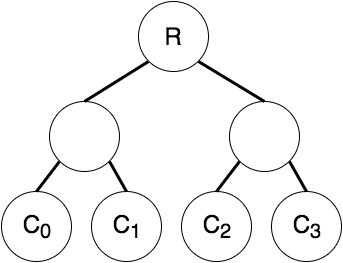
\includegraphics[scale=0.5]{img/naive-parallel}
  \caption{Scheme of merging convex hulls for $k=4$}
  \label{fig:naive-parallel-scheme}
\end{figure}
\fi

The time complexity of this algorithm depends on the size of intermediate convex hulls.
In the worst case scenario the size of the convex hull will be linear to the size of the input.
The time complexity of the algorithm can be estimated as:
$$O(\frac{n}{k}) + O(2\frac{n}{k}) + O(4\frac{n}{k}) + ... + O(k\frac{n}{k}) = O(n)$$
We can see that asymptotically this algorithm in the worst case scenario does not provide any speedup when using more threads.
However, as shown and explained in next sections, this algorithm proved to be quite efficient.

\mypar{{\it Simple} algorithm}
This algorithm is based on computing what part of $C_i$ is also a part of $R$.
The computations are based on the following observation:
\begin{observation}
Let $C_i = \{q_0, q_1, ..., q_{l-1} \},$ where  $q_{j_1}.x < q_{j_2}.x$ for $0 \leq j_1 < j_2 < l$. 
We have that for every $0 \leq j_1 < j_2 < j_3 < l$, if $q_{j_1}, q_{j_3} \in R$, then $q_{j_2} \in R$.
\end{observation}
We will call a point $p$ {\it taken} if and only if $p \in C_i \land p \in R$ for some $i$. 
The above observation means that the points taken from one convex hull form an interval (with regards to their indices).

Computing these intervals can be done by computing the common tangent line of each pair $C_i$ and $C_j$, using the same approach used in {\it Naive} algorithm. 
For given $i$ we can then compute intersection of the intervals computed for $C_i$ and $C_j$ for every $j \neq i$.
Let $[j_1, j_2]$ be the interval of indices corresponding to the calculated intersection.
If $j_1 < j_2$ then this interval corresponds also to the interval of taken points.
However, when $j_1 = j_2$ there might be two possible cases.
They are illustrated in the figure \ref{fig:simple-parallel}.
In the first case we have that the appropriate point is taken, in the second one - it is not.
The difference between these cases is the angle that common tangents lines are forming.
In the first case, when going from left to right the angle between two steepest common lines is less than $\pi$, in the second case it is greater or equal $\pi$.
This means that in the algorithm we need to keep track also of the steepest common tangent lines and use this information for this special case.
Solution for this special case was not presented in $\cite{SimpleParallel}$ and is originally developed by us.

\begin{figure}
\centering
\begin{subfigure}{.3\textwidth}
	\centering
	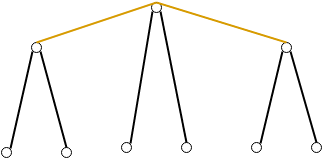
\includegraphics[width=\linewidth]{img/simple-parallel-taking}
	\caption{Point with index $j_1$ is taken}
\end{subfigure}
\begin{subfigure}{.3\textwidth}
	\centering
	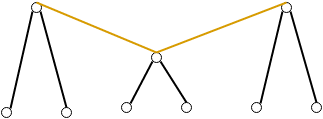
\includegraphics[width=\linewidth]{img/simple-parallel-not-taking}
	\caption{Point with index $j_1$ is not taken}
\end{subfigure}
\caption{Different possibilities for $j_1 = j_2$}
\label{fig:simple-parallel}
\end{figure}

These computations are done in parallel.
Processor $i$ computes all intervals for $C_i$ and $C_j$, where $j = 0, 1, ..., i -1, i+ 1, ..., k - 1$ and then computes their intersection.

The last step consists in moving all taken points to one resulting array.
Firstly, we compute how many points from each convex hull $C_i$ are taken.
Let the result of this computation be: $l_1, l_2, ..., l_{k-1}$.
We can then compute starting positions in the resulting array for each taken points set from one convex hull.
Taken points from $C_i$ should be put at indices from $l_1 + l_2 + ... + l_{i-1}$ to $l_1 + l_2 + ... + l_{i-1} + l_i - 1$.
Calculating these indices can be done using parallel prefix computation.
We later copy taken points to the resulting array in parallel - each processor copies points from its own convex hull.

The time complexity for this algorithm, as shown in \cite{SimpleParallel}, is equal $O(\frac{n}{k} + k(\log \frac{n}{k})^2)$ and the algorithm is optimal for $k \leq \frac{\sqrt{n}}{\log n}$.

\mypar{{\it HullTree} algorithm}
The algorithm is based on a special tree-like structure for keeping points of the convex hull.
Let $n$ denote the number of points in the convex hull.
This data structure allows:
\begin{itemize}
\item creating a new hull tree from a convex hull represented as an array, in $O(n)$ time complexity,
\item accessing leftmost and rightmost point, in $O(\log n)$ time complexity,
\item accessing neighboring (with regards to the position on the convex hull) points, in $O(1)$ time complexity,
\item creating a hull tree consisting of subset of points from the original hull tree that have $x$-coordinate lower than the given one, in $O(\log n)$ time complexity,
\item merging two hull trees, where one of them consists of points that have $x$-coordinate lower than all the points from the second one, in $O(\log n + \log m)$ time complexity, where $n$ and $m$ are the number of points in the hull trees to be merged.
\end{itemize}
The details of the implementation of this data structure are presented in the original paper.

This algorithm uses a divide and conquer approach. 
Let $d = \lceil\frac{n}{k}\rceil$ and $S$ be the current set of input points.
If the size of $S$ is lower or equal than $d$, we execute a sequential version of the algorithm and construct a hull tree based on its result.
Otherwise, we split $S$ into $\sqrt{k}$ equal subsets based on $x$-coordinate: $S_0, S_1, ..., S_{\sqrt{k} - 1}$
\footnote{More precisely, we split into $O(\sqrt k)$ sets. In our implementation for $k \geq 4$ we split into $2^w$ sets, where $w$ is the highest number such that $2^{2w} \leq k$ (for $k = 2$ we split into 2 sets).}.
We then compute recursively convex hull for each subset, which results in having hull trees $HT_i$ corresponding to convex hulls $C_i$ of these subsets.
For each recursive call we assign $\sqrt{k}$ processors to compute this convex hull.

In order to merge $HT_0, HT_1, ..., HT_{\sqrt{k} - 1}$ we perform computations similar to the ones performed in the \textit{Simple} algorithm.
Using $\sqrt{k}^2 = k$ processors we compute for each pair $HT_i$ $HT_j$ ($i \neq j$) common tangent line (for each pair we assign one processor).
It is possible to perform this step efficiently, because our data structure enables us to quickly access neighboring points as well as middle points of given interval of points.
Later we compute the intersection of resulting intervals which results in the intervals of taken points.
If $q_i$ and $q_j$ are the beginning and the end of one of these intervals, we split hull tree first by $q_{i-1}.x$ and discard left convex hull, later by $q_j.x$ and discard right resulting convex hull.
We are left then with hull trees representing only taken points.
We merge these hull trees in a tree-like way (with pairwise merge of hull trees).
These operations are performed in parallel by $\sqrt{k}$ processors and take $O(h + \log k)$ time, where $h$ is the maximum height of considered trees.
Finally, using parallel prefix computation we copy points from the resulting hull tree into the resulting array.

The time complexity for this algorithm, as shown in \cite{HullTree}, for $k \leq \frac{n}{\log n}$ is equal $O(\frac{n}{k})$ and is optimal.

\section{Experimental results}\label{sec:exp}

In order to evaluate the efficiency of our proposed algorithms, we tested them on sets of randomly generated points with different geometric shapes: square, disk and circle.

Regarding scalability we tested both weak and strong scaling, changing the input size and the number of operating threads.

Concerning correctness we compared our results with the ones obtained using the Graham-Andrew's algorithm implementation available in the library \textit{CGAL}\cite{CGAL}.

\mypar{Experimental setup}
The platform we tested our algorithms on mounts Intel Xeon Phi coprocessors.
They are based on the Intel Many Integrated Core (MIC) architecture.
The following characteristics have been retrieved by reading from \path{/proc/cpuinfo} file:

\begin{table}[!ht]
\begin{tabular}{|c|c|}
\hline Number of cores			& 61\\
\hline Total threads				& 244\\
\hline Model name				& Intel Xeon Phi 7100\\
\hline CPU Frequency [MHz]		& 1238.094\\
\hline Cache size [KB]			& 512\\
\hline Peak Performance [GFlops]	& 1208\\
\hline Peak memory bandwidth [GB/s]		& 352\\
\hline
\end{tabular}
\caption{Intel Xeon Phi coprocessors specifications \cite{XeonPhi}}
\end{table}

Our implementations are written in \textit{C++11} and make use of \textit{OpenMP} ver 4.0 \cite{OpenMP} for shared memory multithreading.
Our applications were compiled using \textit{icc} version 15.0.0 with the flag \textit{-O2} using also the -mmic flag to fit the architecture.

This is roughly how our experiments worked:
first of all we fixed a shape and a number of points to be generated. Then we randomly generated the chosen point set and executed each algorithm with each desired number of threads on that point set, collecting results in logfiles. We measured two time intervals: \textit{mid} (the time needed for the first part of the algorithms that is the separated computing of convex hulls) and \textit{end} (the time needed for merging results).

In order to have reliable experiments we repeated this process 100 times for each chosen combination of number of input points and shape.

This whole process was done for 10$^4$, 10$^5$, 10$^6$ and 10$^7$ points with integral coordinates and different $x$-coordinates generated in a range $R$ of 10$^9$ and as shapes we used square, disk and circle in the following way:\\
{\bf Square}: Randomly generated points with coordinates in the range [$-R$,$R$]\\
{\bf Disk}: Randomly generated points with coordinates in the range [$-R$,$R$]. Points not included in the disk with radius R and center (0,0) were removed and regenerated.\\
{\bf Circle}: Randomly generated angles $\theta_n$ and created the points ($\lfloor R \cos(\theta_n)\rfloor$, $\lfloor R \sin(\theta_n)\rfloor$). Please note that while points generated with square and disk constitute dense figures, with circle points lay only on the border of the shape.

These shapes were chosen because of the difference in the resulting hulls.
With square, in fact, resulting hulls are very small, while with the circle almost every input point is part of the final hull (some of the points will be excluded because of approximation of integers) and for disk resulting hulls have intermediate size.

\mypar{Results}
Here we show how our algorithms perform under different configurations and with weak and strong scaling.
The results plotted are statistical data taken from the 100 different repetitions performed for each configuration (input shape, input size, algorithm and number of processing threads): arithmetic mean for execution times and harmonic mean for speedup.
These always come along with 95\% confidence intervals (even though very often the confidence interval is too small to be noticable).

Results obtained with disks as input are not shown because they were close to identical to the squares' ones.

As a base case for speedup plots we used our implementation for \textit{Andrew's Monotone Chain}, which is also used inside our parallel algorithms.

\mypar{Changing input size for fixed number of threads}
Here we analyze the results of our algorithms when changing input size from 10$^4$ to 10$^7$ points. 
We show performance with 8 processing threads to represent the trends of the algorithms, which are generally the same (with different speedups) for the tested number of threads.

\begin{figure}[!ht]\centering
  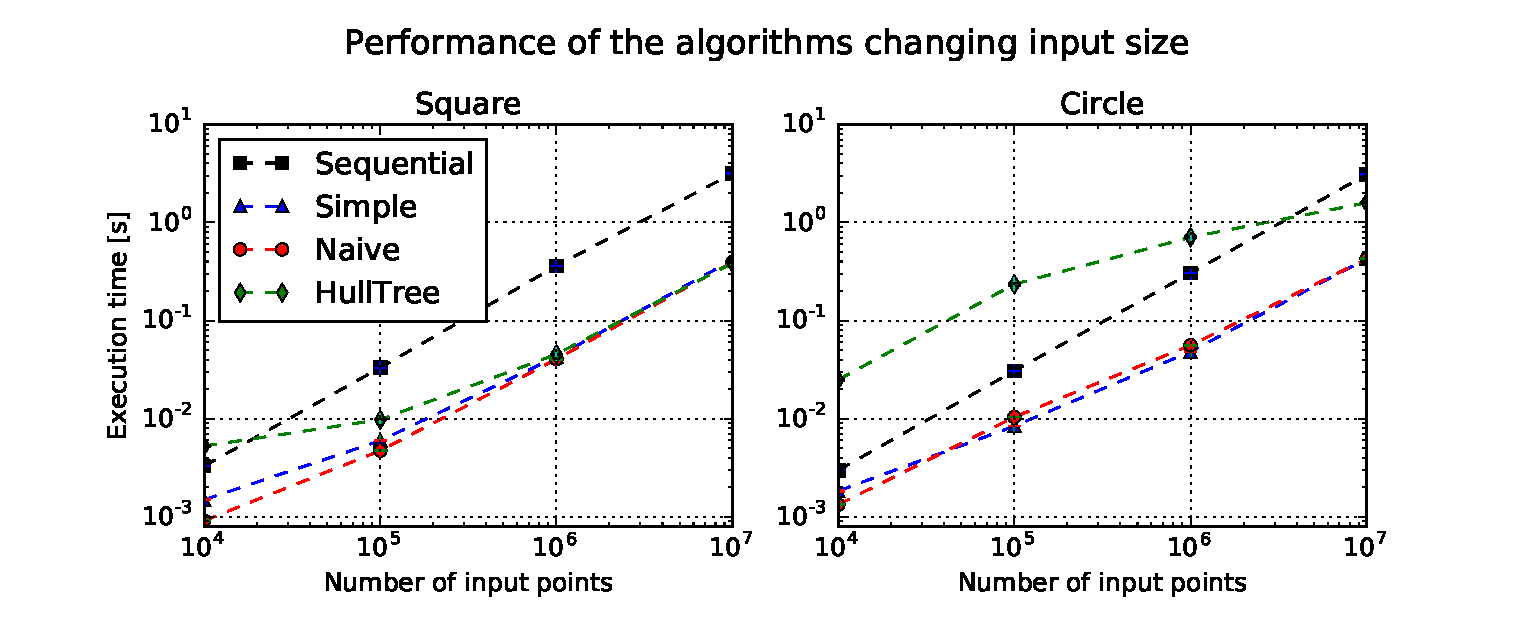
\includegraphics[scale=0.33]{./plots/time_points.eps}
  \caption{Comparison of the execution times of the three parallel algorithms using 8 threads and the sequential version, changing input size for square and circle\label{Input size time}}
\end{figure}

For the sequential versions the growth in execution time when increasing the number of input points is linear for all the selected shapes.
Concerning the parallel algorithms they have similar trends except for \textit{HullTree}, that performs significantly worse for small input sets [Plot \ref{Input size time}], especially with the circle: \textit{HullTree}'s performance is even worse than the sequential one.
This is due to the creation of the data structure that for a high number of resulting points (recall that for circle almost every generated point is part of the final convex hull) needs a lot of time.

\begin{figure}[!ht]\centering
  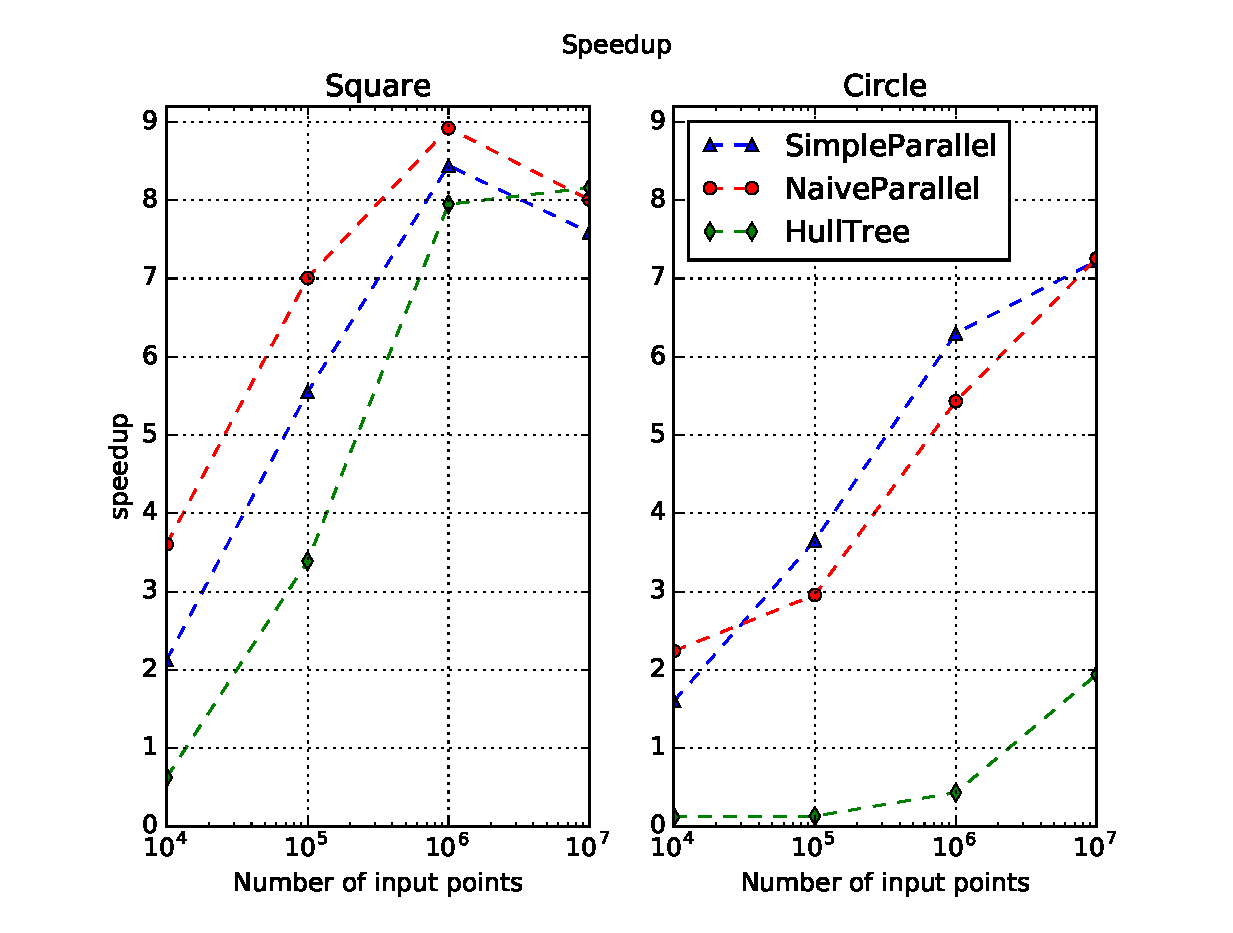
\includegraphics[scale=0.33]{./plots/speedup_points.eps}
  \caption{Speedup comparison of the three algorithms for 8 threads changing input size for square and circle\label{Input size speedup}}
\end{figure}

Looking at the speedup plots [Plot \ref{Input size speedup}] the general trend is a growth in efficiency when increasing the size of the input set for the two shapes.

We notice a superlinear speedup for 10$^6$ points (around 9 for \textit{Naive} and 8.5 for \textit{Simple}) and 10$^7$ points (slightly above 8 for both \textit{Simple} and \textit{HullTree}).
We obtained superlinear speedup thanks to caching: splitting the input set into smaller subsets assigned to processors makes the subset fit better into cache, allowing faster accesses to the points.

A good performance of \textit{Naive} algorithm can be attributed to the used vectorization.
The main factor in the complexity of this algorithm was copying the points to the resulting array during the merge of convex hulls.
Vectorization used on Xeon Phi speeds up this process significantly and therefore the algorithm performs much better than the calculated time complexity might suggest.

The bad performance of the \textit{HullTree} algorithm can be attributed to the necessity of dynamically allocating a lot of data connected with the underlying data structure.
Hull tree nodes are dynamically allocated to not-continuous memory, which makes the algorithm slower.
It was necessary to allocate first some continuous memory by the thread creating this data structure, which provided some increase in the performance.

\mypar{Changing number of threads for fixed input}
Here we analyze the performance of our algorithms with different numbers of processing threads under a fixed input of 10$^6$ and 10$^7$ points.

\begin{figure}[!ht]\centering
  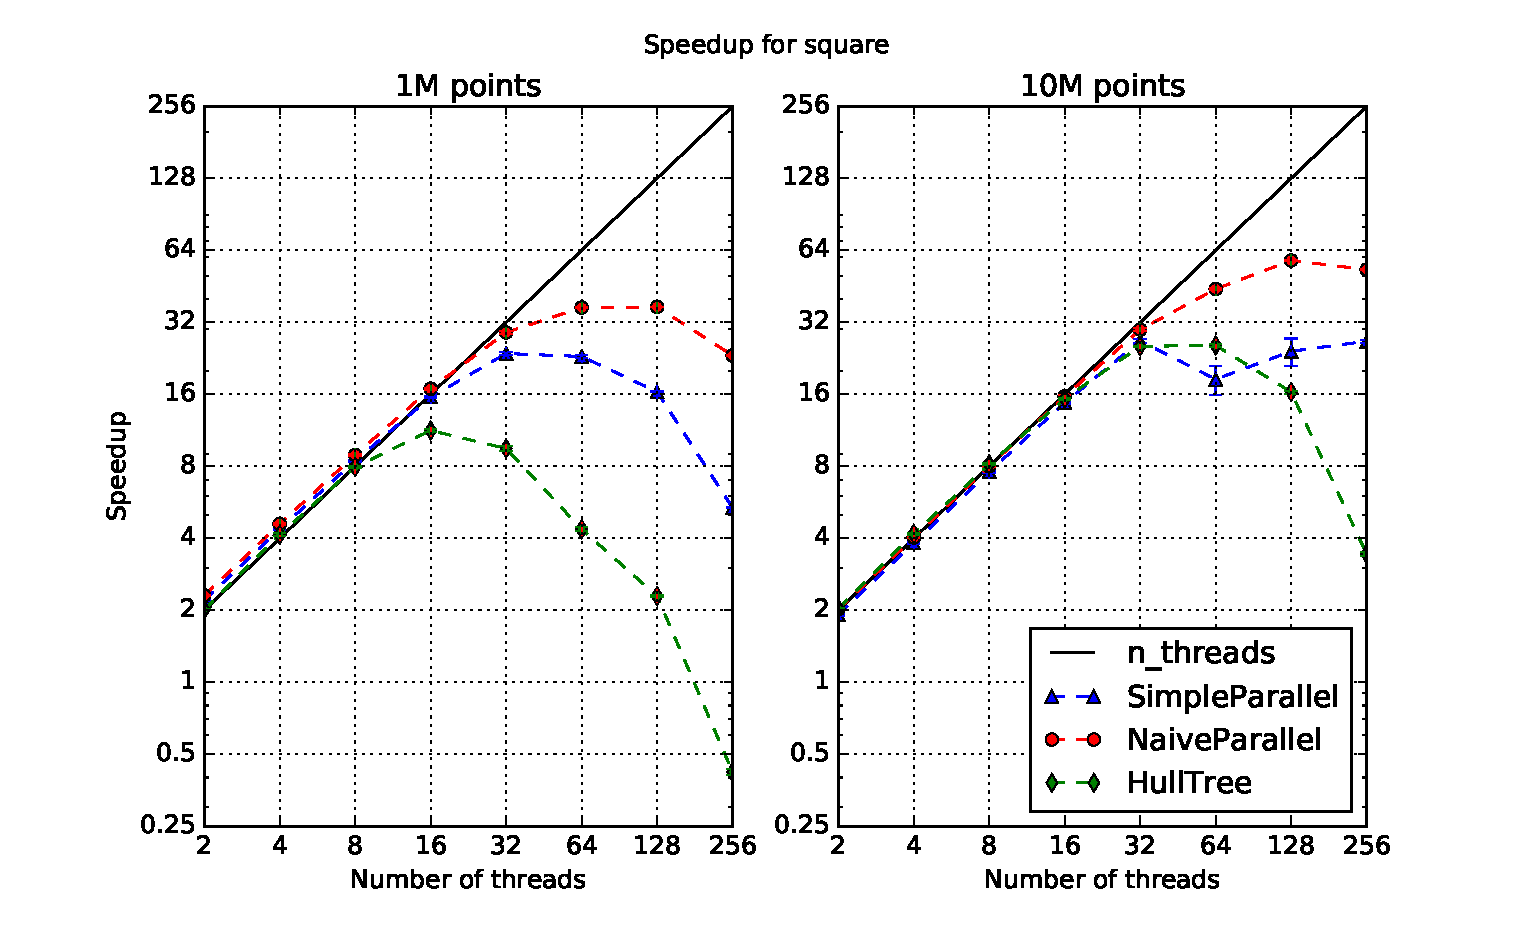
\includegraphics[scale=0.33]{./plots/speedup_xeon_square_fixed_points.eps}
  \caption{Speedup of the algorithms with the given number of threads with a square for 10$^6$ [avg. sequential execution time: 0.361s] and 10$^7$ [avg. sequential execution time: 3.1561s] points\label{Threads speedup square}}
\end{figure}

For square and disk we notice similar trends [Plot \ref{Threads speedup square}] speedup close to linear or even superlinear up to around 16 threads for 10$^6$ points and 32 for 10$^7$ points, then a general decrease in efficiency growth up to a point where our algorithms stop scaling and the speedup starts decreasing.

We can notice that that point is shifted to a higher number of threads when the input set is bigger.
Clearly the larger the number of points, the higher the efficiency obtained by splitting the point set among threads.
After that point, the overhead added by parallelism outbalances the benefits introduced by having more processing units.

This overhead is related both to the operating system, that has to create, allocate and manage a high number of threads, and to the algorithms themselves:
in fact for a large number of threads, while the first part of the algorithms (separately compute convex hulls on split point sets) becomes very fast, the merging itself takes more time and the two processes start becoming unbalanced.

\begin{figure}[!ht]\centering
  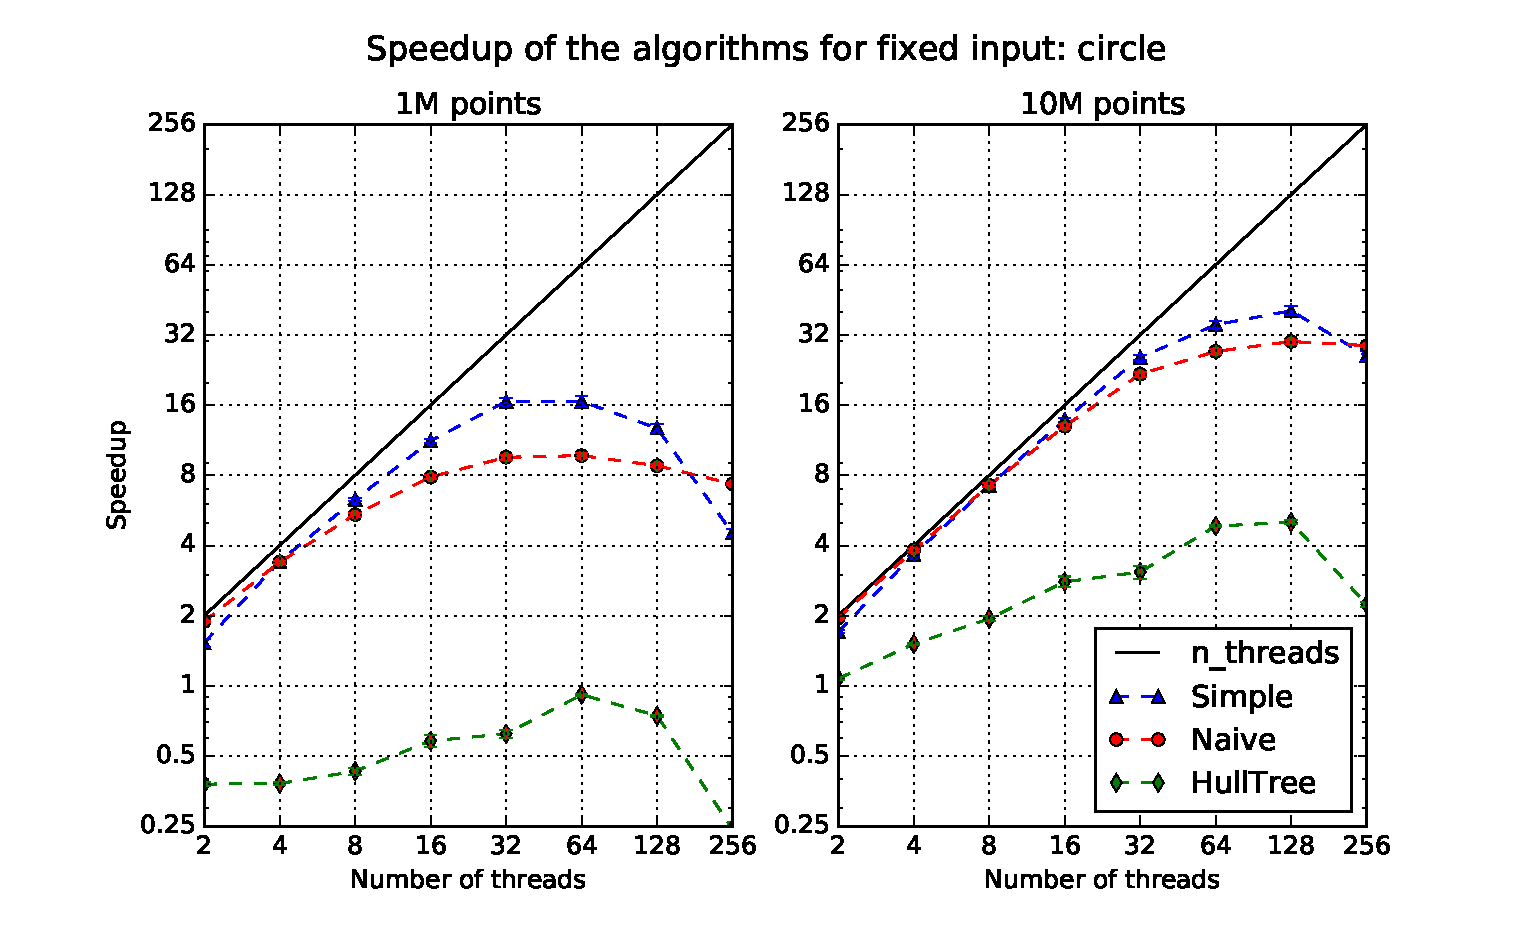
\includegraphics[scale=0.33]{./plots/speedup_xeon_circle_fixed_points.eps}
  \caption{Speedup of the algorithms with the given number of threads with a circle for 10$^6$ [avg. sequential execution time: 0.304s] and 10$^7$ [avg. sequential execution time: 3.085s] points\label{Threads speedup circle}}
\end{figure}

For circle [Plot \ref{Threads speedup circle}] the situation is again more complicated, since the \textit{HullTree} algorithm has a very bad performance, but the trend is very similar with a fast increase in efficiency followed by a close-to-steady state and a decrease in efficiency for a large number of threads.
Quantitatively the overall efficiency of the parallel algorithms is lower than the one obtained with the square and that's probably because the more memory accesses needed and the parallel overhead make the algorithms behave worse.

\mypar{Behavior with not optimal number of threads}
For a number of threads that is not a power of 2, because of its implementation, \textit{HullTree} algorithm behaves like the closest lower power of two (i.e. with 35 threads it behaves like if it had 32).

\textit{Simple} and \textit{Naive} algorithms, instead, still work well: the former because it's not related to powers of 2 in any one and the latter thanks to the creation of dummy nodes. Their performance is consistent, as shown in plot \ref{Speedup Total}, having little drops around multiples of 61 threads, where we start having hyperthreading.

\begin{figure}[!ht]\centering
  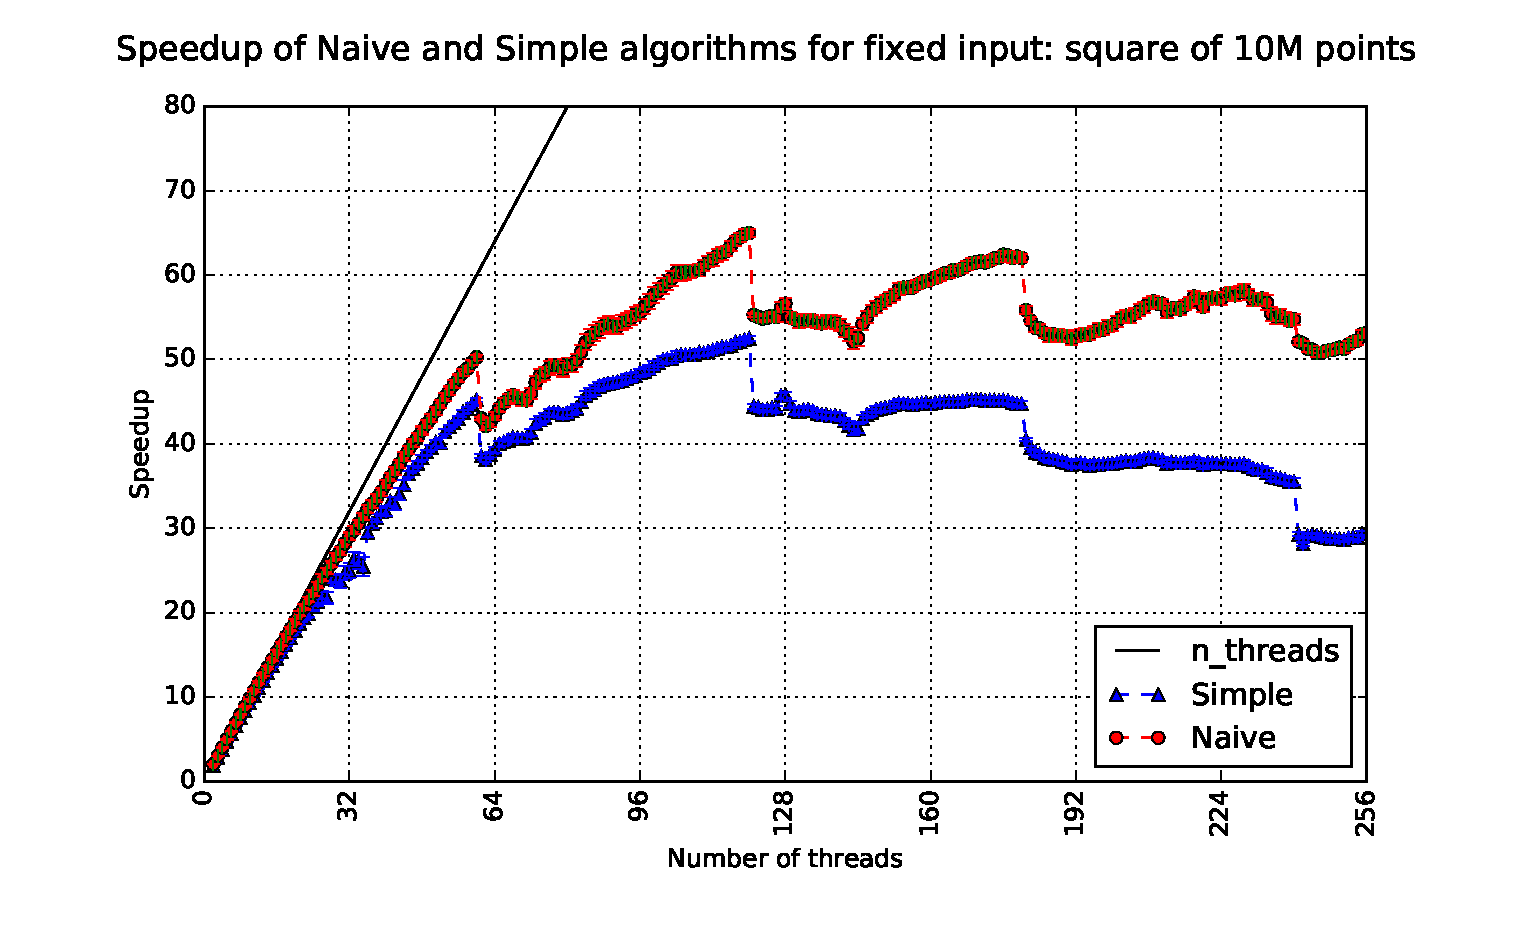
\includegraphics[scale=0.3]{./plots/total_speed.eps}
  \caption{Speedup of Simple and Naive algorithms for a square of 10$^7$ points [avg. sequential execution time: 3.1561s]\label{Speedup Total}}
\end{figure}

\section{Conclusions}

We implemented three parallel algorithms for solving the convex hull problem and as a general remark we believe that all the considered algorithms are valid and allow good performance under different conditions (input size, shape and number of processing threads).
One of the algorithms (\textit{HullTree}), however, doesn't work nicely with very large resulting hulls (like with circles as input sets).

We were able to obtain superlinear speedup using randomly generated points in a square and close to linear with two of the three algorithms using a circle as input.

Generally speaking, we could say the parallelization of the convex hull problem allows significant improvements in performance with larger input sets and with a not-too-large number of processing threads.

Even though we only considered square, disk and circle as shapes for the input set, these algorithms can be used for any ordered input set with distinct $x$-coordinate and their performance should be similar to the one we had with the analyzed shapes (i.e. similar to circle's one if most of the points in the input set takes part to the final hull, else similar to disk and square's ones).

Regarding applications to different dimensions, we believe that the concept of \textit{Naive} algorithm can be adapted to a 3D space by using gift wrapping algorithm instead of common tangent line algorithm.
The other two algorithms, however, have a 2D-specific approach and cannot be easily adapted to a higher number of dimensions.

% References should be produced using the bibtex program from suitable
% BiBTeX files (here: bibl_conf). The IEEEbib.bst bibliography
% style file from IEEE produces unsorted bibliography list.
% -------------------------------------------------------------------------
\bibliographystyle{IEEEbib}
\bibliography{bibl_conf}

\end{document}

